\chapter{Referencial Teórico}
\label{chap:refteorico}

Nesta seção será apresentada o embasamento teórico para desenvolvimento do projeto.

%================================================================================
\section{Sistemas de Visão Computacional}
\label{sec:sistemasVisaoArtificial}

Um sistema de visão computacional é composto por etapas, sendo elas: definição do problema, aquisição da imagem, pré-processamento, segmentação, identificação do objeto e reconhecimento de padrões, como visto na Figura~\ref{fig:acoesProcImagem}.

\begin{figure}[!hbtp]
  \centering
   \caption{Ações de Aquisição e Processamento de Imagem.}
    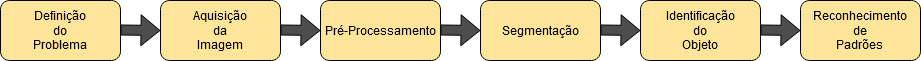
\includegraphics[width = 0.8\textwidth]{Caps/Figs/ref-teorico/acoes-procImagem.jpg}
   \label{fig:acoesProcImagem}
    \fonte{Autor}
\end{figure}

\subsection{Definição do Problema}
\label{subsec:defProblema}

Para \citeauthor{rogeralex1999} (\citeyear{rogeralex1999}), a primeira etapa do processo é a definição do problema, ou seja, qual é o objetivo que o sistema deve cumprir. Este pode ser a identificação de peças numa esteira rolante, a identificação de impressões digitais ou o reconhecimento de obstáculos na trajetória de um robô móvel. Se o sistema tiver sido bem planejado, chega-se a última etapa do processo, que é o resultado, ou seja, qual é a peça, a quem pertence a impressão digital ou qual é o obstáculo do robô.

\subsection{Aquisição da Imagem}
\label{subsec:aquisImagem}

Nesta etapa necessita-se de um dispositivo sensível a faixa do espectro eletromagnético desejado, também conhecido como câmera. Estes equipamentos que compõe o ambiente produzem em sua saída um sinal elétrico proporcional a quantidade de energia captada. Esse sinal elétrico, precisa então passar por um conversor analógico-digital para que possa ser processado pelo computador \cite{rogeralex1999}.

\subsection{Pré-processamento da Imagem}
\label{subsec:preProcImagem}

Após digitalizar e armazenar a imagem em um computador, as técnicas de pré-processamento são usadas para aprimorar a qualidade de uma imagem, corrigindo iluminação, contraste, distorções e nitidez~\cite{rudek2001visao}.

Essas operações podem ser realizadas tanto no domínio espacial quanto no domínio da frequência. O domínio espacial refere-se ao próprio plano da imagem e é caracterizado pela manipulação direta dos pixels. As técnicas de processamento no domínio da frequência são baseadas na manipulação da Transformada de Fourier da imagem~\cite{rogeralex1999}.

\subsection{Segmentação da Imagem}
\label{subsec:segImagem}

\citeauthor{heinen2004navegaccao} (\citeyear{heinen2004navegaccao}) afirma que em processamento de imagens, segmentar consiste em identificar e extrair estruturas homogêneas presentes em uma cena, sendo a eficiência deste processo diretamente relacionada ao desempenho final da análise automática de imagens. É importante enfatizar que essa é uma etapa crítica do processo.

Esta técnica é utilizada para reduzir o esforço computacional, reduzindo as informações da imagem. Para~\citeauthor{rudek2001visao} (\citeyear{rudek2001visao}), a ideia utilizada na segmentação (\textit{thresholding}) é dividir a imagem em regiões que correspondem a unidades estruturais da cena, ou que distinguem os objetos de interesse, separando os objetos da imagem (\textit{foreground}) das informações de fundo da imagem (\textit{background}). Com esta abordagem, minimiza-se o tamanho do espaço de onde as informações são retiradas, diminuindo o esforço computacional necessário para tratar a imagem.

A dificuldade normalmente encontrada está no fato de não haver conhecimento a priori do número e tipo de estruturas presentes na imagem. Estas são identificadas a partir de características como forma, geometria, topologia, textura, cor ou brilho, sendo escolhidas aquelas que possibilitam melhor distinção~\cite{heinen2004navegaccao}.

\subsection{Identificação do Objeto}
\label{subsec:idObjeto}

Visto que os elementos de interesse da imagem foram individualizados, deve-se determinar a melhor forma de representá-los, isto é, se apenas o seu contorno já contém a informação necessária ou se todos os pixels são necessários para a identificação do objeto. Portanto, deve-se determinar características do objeto que possam contribuir para a sua identificação.

\citeauthor{rudek2001visao} (\citeyear{rudek2001visao}) afirma que devido a uma variedade de razões, os dados de imagens usados na entrada de um sistema de visão, nem sempre são perfeitos. Os problemas que frequentemente ocorrem estão relacionados com a oclusão, onde um objeto pode estar parcialmente escondido atrás de outro objeto. 

De forma análoga, a perda de informações ou deformações, podem ser ocasionadas por ruídos na imagem devido a condições anormais de iluminação, defeitos de digitalização, e de resultados ineficientes de algoritmos de segmentação~\cite{beis1999indexing}.

\subsection{Reconhecimento de Padrões}
\label{subsec:recPadroes}

As técnicas de reconhecimento de padrões, tratam da identificação de partes da imagem que possuem semelhanças. Uma grande quantidade de ferramentas matemáticas e computacionais, tem sido desenvolvidas para permitir que objetos possam ser extraídos e agrupados em classes específicas de informações. Uma boa representação da forma do objeto, gera facilidades para que ele seja armazenado, transmitido, comparado, reconhecido ou mesmo entendido. A representação deve ser gerada de acordo com regras simples e precisas. Geralmente uma forma é descrita em termos de número de componentes, primitivas e relacionamentos entre estes componentes~\cite{rudek2001visao}.

%================================================================================
\section{Métodos de Visão Computacional}
\label{sec:openCV}

Diversas técnicas para a segmentação de imagens em sistemas de visão computacional foram desenvolvidas de acordo com o objetivo do RMA. Algumas utilizam duas câmeras e outros apenas uma, e estas podem estar dispostas fixas ao robô ou no ambiente. \citeauthor{andrade2006sistema} (\citeyear{andrade2006sistema}), propõe um sistema onde duas câmeras são dispostas no ambiente e executam uma triangulação. Ainda cita que, \citeauthor{souza2003desenvolvimento} (\citeyear{souza2003desenvolvimento}) propõe um sistema baseado na limiarização das cores dos componentes da imagem através das proporções de seus componentes vermelho, verde e azul, e; \citeauthor{penharbel2004filtro} (\citeyear{penharbel2004filtro}), utilizam os componentes vermelho, verde e azul dos pixels para obter o tom, saturação, e a intensidade das cores, a fim de efetuar a limiarização sobre este último espaço de valores.

\subsection{Triangulação com Câmeras no Ambiente}
\label{subsec:triangulacao}

Uma das propriedades mais relevantes deste sistema é o fato de que ele opera extraindo imagens a partir de duas câmeras. Uma delas é posicionada perpendicularmente ao plano de operação do robô e outra de forma inclinada. O interesse em uma segunda câmera com posição inclinada é, além de tornar a análise da cena mais robusta, tornar possível a detecção de obstáculos finos e alongados verticalmente, o que poderia ser tratado como ruído e passar despercebido no sistema de visão \cite{andrade2006sistema}.

A princípio, a imagem capturada pela câmera é pré-processada pelo sistema, visando eliminar seu fundo. Para isso, pode-se utilizar técnicas de limiarização, que é o processo de segmentação de imagens que se baseia na diferença dos níveis de cinza que compõe diferentes objetos de uma imagem.

\citeauthor{andrade2006sistema} (\citeyear{andrade2006sistema}) explicam que, no pré-processamento das imagens seguintes, a cor a ser tida como padrão durante a rotulação dos pixels é definida como a média temporal de todas as cores obtidas até então. Essa medida evita que mudanças bruscas no ambiente afetem o funcionamento do sistema. A segmentação do robô também utiliza a limiarização, e são segmentados os pixels cuja distância no espaço tricromático a cor de frente ou a de fundo do robô (definidas pelo usuário na inicialização do sistema) é inferior a um limiar. A área do robô é calculada pelo somatório dos seus pixels, sua posição é definida como sendo as coordenadas de seu centro de área, e sua orientação é definida como o ângulo formado pela semi-reta que tem como origem o centro de área da região do fundo do robô e passa pelo centro de área da região de sua frente. O processo utilizado na verificação de obstáculos é baseado em um sonar visual, onde são utilizados 18 feixes que saem do centro de área do robô em diferentes ângulos e vão percorrendo a imagem pixel a pixel. A varredura de cada feixe termina quando ele encontra um obstáculo ou quando atinge um dos limites da imagem. As coordenadas dos pontos de parada de cada feixe são guardadas em um vetor, que é passado para o sistema de controle juntamente com as características do robô.

O sistema desenvolvido por \citeauthor{andrade2006sistema} (\citeyear{andrade2006sistema}), pode ser visto na Figura~\ref{fig:triangulacao}.

\begin{figure}[!hbtp]
  \centering
   \caption{Processo de Extração de Características.}
    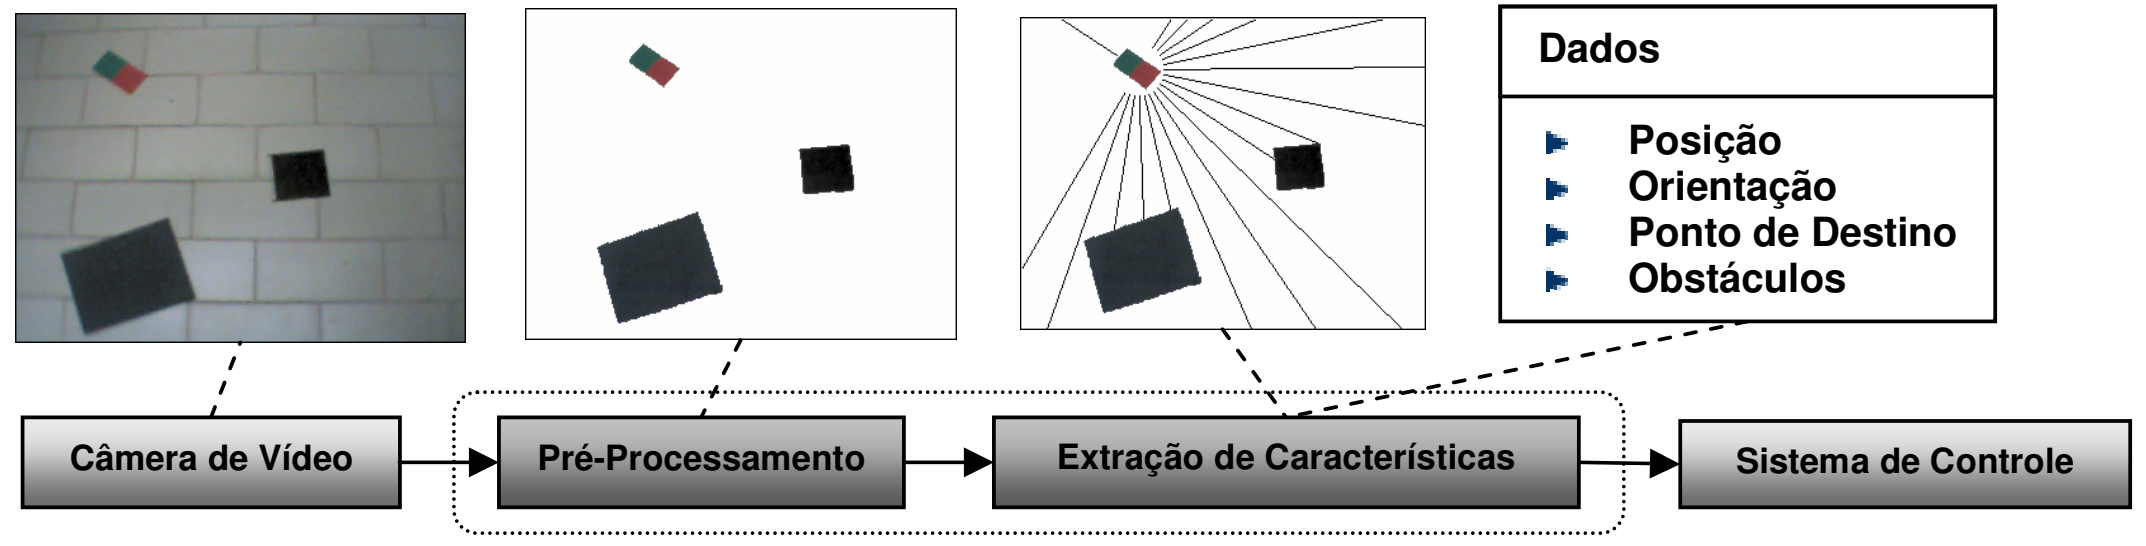
\includegraphics[width = 0.8\textwidth]{Caps/Figs/ref-teorico/triangulacao.png}
   \label{fig:triangulacao}
    \fonte{\citeauthor{andrade2006sistema} (\citeyear{andrade2006sistema})}
\end{figure}


\subsection{RGB}
\label{subsec:rgb}

\subsection{HSV}
\label{subsec:hsv}


%================================================================================
\section{OpenCV}
\label{sec:opencv}

A OpenCV (\textit{Open Source Computer Vision Library})


 
